\documentclass[10pt, a4paper]{article}
% \usepackage{newtxtext,newtxmath}
\usepackage{geometry}
\usepackage{graphicx}
\usepackage{hyperref}
\usepackage{array}
\usepackage{booktabs}
\usepackage{tikz}
\usepackage{enumitem}



% --- Layout & links ---
\usepackage[margin=1.5in]{geometry}
\usepackage{hyperref}
\hypersetup{colorlinks=true,linkcolor=black,urlcolor=blue}
\usepackage{enumitem}

% --- Use local EB Garamond font ---
\usepackage{fontspec} % Para usar fuentes OpenType y TrueType
\usepackage{libertinust1math}
\setmainfont{EB Garamond}[
    UprightFont = * Regular,
    ItalicFont = * Italic,
    BoldFont = * SemiBold,
    BoldItalicFont = * SemiBold Italic,
]

% --- Justification ---
\usepackage{ragged2e}
\justifying

% --- Line spacing ---
\usepackage{setspace}
\setstretch{1.25}

% --- Paragraph spacing ---
\setlength{\parskip}{0.2em}

% --- Page layout ---
\usepackage{fancyhdr}
\pagestyle{fancy}
\fancyhf{}
% Elegant header: course title left, document title center, page number right
\fancyhead[L]{\small\textsc{AI in Financial Services}}
% \fancyhead[C]{\small\textbf{LumenCash: Embedded Finance}}
\fancyhead[R]{\small\thepage}
\vspace{1em}
\renewcommand{\headrulewidth}{0.05pt}


% --- Do not number the first page ---
\thispagestyle{empty}


% --- Itemize settings ---
\setlist{nosep,leftmargin=*,labelsep=0.5em}

% --- Title ---

\begin{document}
\vspace*{-5em}
\begin{center}
   \LARGE{\textbf{Artificial Intelligence in Algorithmic Trading: 
An Extended Guide for Financial Services}} 
\end{center}

\section*{Introduction}
Algorithmic trading (\emph{algo trading}) relies on automated systems to execute orders at speed and scale. With Artificial Intelligence (AI), strategies have evolved from static rules to adaptive, data-driven approaches capable of learning from vast and diverse sources. This guide explains how AI is applied in trading, what data and models are used, the key benefits and risks, ethical challenges, and real-world cases (Two Sigma, Kavout). Visual figures and tables support clarity.

\section*{How AI Works in Algorithmic Trading}
A modern AI trading workflow involves:
\begin{enumerate}[leftmargin=*,itemsep=2pt]
  \item \textbf{Data ingestion}: tick-level prices, order book depth, volumes, macro releases, news and sentiment, alternative data (weather, satellite imagery, shipping flows), and corporate events.
  \item \textbf{Preprocessing}: cleaning, normalization, time alignment, imputation, feature engineering (returns, realized volatility, order-flow imbalance, textual embeddings).
  \item \textbf{Modeling}: supervised/self-supervised learning for trading signals; unsupervised for anomaly and regime detection; reinforcement learning for sequential decision-making.
  \item \textbf{Execution}: mapping signals into orders, smart order routing, controlling slippage and transaction costs; continuous retraining and feedback loops.
\end{enumerate}

\begin{center}
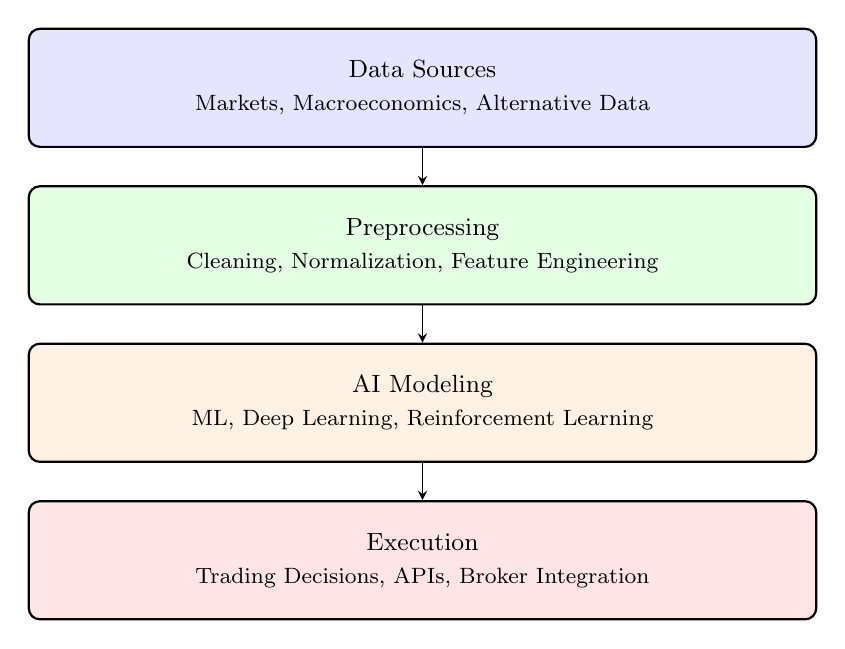
\begin{tikzpicture}[>=stealth, thick]
\tikzset{
  box/.style={
    draw, rectangle, rounded corners,
    minimum width=10cm, minimum height=1.5cm,
    align=center
  }
}
\node[box, fill=blue!10]   (data) at (0, 0)    {\small Data Sources\\ \footnotesize Markets, Macroeconomics, Alternative Data};
\node[box, fill=green!10]  (prep) at (0,-2.0)  {\small Preprocessing\\ \footnotesize Cleaning, Normalization, Feature Engineering};
\node[box, fill=orange!10] (model) at (0,-4.0) {\small AI Modeling\\ \footnotesize ML, Deep Learning, Reinforcement Learning};
\node[box, fill=red!10]    (exec) at (0,-6.0)  {\small Execution\\ \footnotesize Trading Decisions, APIs, Broker Integration};

\draw[->, line width=0.5pt] (data) -- (prep);
\draw[->, line width=0.5pt] (prep) -- (model);
\draw[->, line width=0.5pt] (model) -- (exec);
\end{tikzpicture}

\vspace{0.3cm}
\textit{Figure 1: AI trading pipeline.}
\end{center}

\section*{Data Types and AI Models}
\textbf{Data}: tick-by-tick trades, level-2/3 order books, OHLCV bars, corporate actions, macro calendars, real-time news and social media (text), PDF filings (NLP), satellite images (computer vision), and latency telemetry.\\[2pt]
\textbf{Models}:
\begin{itemize}[leftmargin=*,itemsep=2pt]
  \item \textbf{Supervised}: logistic regression, boosting, LSTMs, CNNs, Transformers for time series; mid-price movement prediction.
  \item \textbf{Unsupervised/self-supervised}: autoencoders, contrastive learning embeddings, clustering for regime detection, change-point analysis.
  \item \textbf{Reinforcement Learning}: contextual bandits for execution venue choice; DQN/Policy Gradient/PPO for inventory control and market making; reward functions include PnL, risk, and transaction costs.
  \item \textbf{NLP/Vision}: sentiment classification with LLMs, retrieval-augmented generation (RAG) for financial text; satellite-based asset monitoring.
\end{itemize}
\section*{Reinforcement Learning in Trading}
Unlike supervised models trained on labeled data, RL agents learn policies by interacting with a market environment and receiving feedback.

\begin{center}
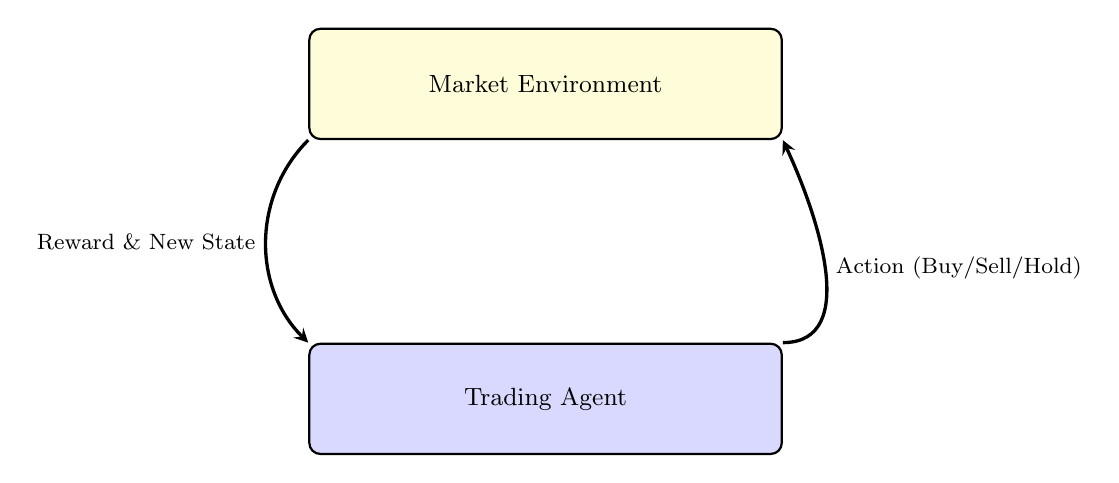
\begin{tikzpicture}[>=stealth, thick]
\tikzset{
  box/.style={
    draw, rectangle, rounded corners,
    minimum width=6cm, minimum height=1.4cm,
    align=center
  }
}

% Nodes
\node[box, fill=blue!15]   (agent)  at (0, -2)  {\small Trading Agent};
\node[box, fill=yellow!15] (market) at (0,  2)  {\small Market Environment};

% Curved arrows forming a loop
\draw[->, line width=1.2pt] (agent.north east) to [out=0,in=-2225] node[midway, right]{\footnotesize Action (Buy/Sell/Hold)} (market.south east);
\draw[->, line width=1.2pt] (market.south west) to [out=-135,in=135] node[midway, left]{\footnotesize Reward \& New State} (agent.north west);

\end{tikzpicture}

\vspace{0.5cm}
\textit{Figure 2: Reinforcement learning loop for trading decisions.}
\end{center}

The policy $\pi(a|s)$ maximizes $\mathbb{E}[\sum_{t}\gamma^t R_t]$, with rewards adjusted for drawdowns, VaR, and execution costs. Simulation and market replay environments reduce overfitting risk.


\newpage
\section*{Technical Architecture}
Deploying AI in trading requires an end-to-end system:
\vspace{0.3cm}
\begin{center}
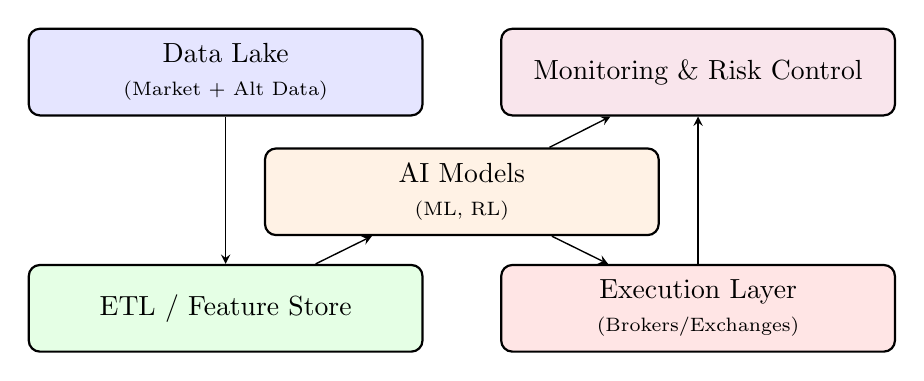
\begin{tikzpicture}[>=stealth, thick, scale=1, every node/.style={transform shape}]
\tikzset{
  box/.style={
    draw, rectangle, rounded corners,
    minimum width=5cm, minimum height=1.1cm,
    align=center
  }
}
\node[box, fill=blue!10]  (lake) at (-3,  2.0) {Data Lake \\ \scriptsize (Market + Alt Data)};
\node[box, fill=green!10] (etl)  at (-3, -1.0) {ETL / Feature Store};
\node[box, fill=orange!10] (model) at (0, 0.48) {AI Models \\ \scriptsize (ML, RL)};
\node[box, fill=red!10]    (exec)    at (3,  -1.0) {Execution Layer \\ \scriptsize (Brokers/Exchanges)};
\node[box, fill=purple!10] (monitor) at (3,  2.0) {Monitoring \& Risk Control};

\draw[->, line width=.5pt] (lake) -- (etl);
\draw[->, line width=.5pt] (etl)  -- (model);
\draw[->, line width=.5pt] (model) -- (exec);
\draw[->, line width=.5pt] (model) -- (monitor);
\draw[->, line width=.5pt] (exec) -- (monitor);
\end{tikzpicture}

\vspace{0.6cm}
\textit{Figure 3: Technical architecture for AI-enabled trading.}
\end{center}

\section*{Benefits vs Risks}
\begin{center}
\small
\renewcommand{\arraystretch}{1.25}
\begin{tabular}{p{6cm} p{6cm}}
\toprule
\textbf{Benefits} & \textbf{Risks / Challenges} \\
\midrule
Ultra-fast execution (milliseconds) & Overfitting on historical datasets \\
Adaptive strategies in volatile regimes & Sensitivity to noisy signals \\
Pattern discovery in heterogeneous data & Opaque decision-making (black box) \\
Operational cost efficiency & Ethical and regulatory scrutiny \\
Scalability across asset classes & High infrastructure and latency costs \\
\bottomrule
\end{tabular}

\vspace{0.25cm}
\textit{Table 1: Comparative overview of AI benefits and risks.}
\end{center}

\section*{Ethical and Governance Considerations}
\begin{itemize}[leftmargin=*,itemsep=2pt]
  \item \textbf{Transparency and explainability}: model cards, data lineage, traceable signals for audit.
  \item \textbf{Systemic risk}: kill switches, circuit breakers, stress testing under extreme regimes.
  \item \textbf{Fairness and manipulation}: avoiding strategies that amplify volatility or create unfair advantages.
  \item \textbf{Privacy and compliance}: respecting data rights, licenses, and personally identifiable information (PII).
\end{itemize}

\newpage
\section*{Real-World Examples}
\paragraph{Two Sigma: Alternative Data and Market Predictions.}
This quantitative hedge fund integrates financial and alternative datasets (including weather and sentiment) with machine learning at scale. Models generate multi-asset predictive signals, exemplifying how AI converts heterogeneous data into operational alpha.
\paragraph{Kavout: Kai Score.}
Kavout assigns predictive ``Kai Scores'' to equities using thousands of features. Investors use these scores for systematic stock screening, blending AI analytics with human oversight.

\section*{Conclusion}
AI has reshaped algorithmic trading with speed, adaptability, and non-trivial pattern recognition. Value depends on robust data pipelines, rigorous validation, cost-aware execution, and strong governance. Institutions that balance innovation with oversight will capture sustainable advantage without undermining market stability.

\newpage
\section*{Part 2: Reflection on AI in Writing (Option A)}
\textbf{Tasks using AI:} text structure and generating figures. \\
\textbf{Engagement with AI output:} I revised and adapted drafts, correcting diagrams, balancing tables, and expanding technical depth. \\
\textbf{Efficiency gains:} AI accelerated drafting, maintained terminological consistency, and helped iterate visual elements until they were clear. \\
\textbf{Limitations:} AI sometimes produced generic text or overlooked financial nuances (e.g., transaction costs, regime shifts). \\
\textbf{Future role:} AI tools will continue to support technical briefings, LaTeX templates, and executive summaries. However, human oversight will remain essential for credibility, compliance, and accountability.

\end{document}
